\begin{figure}[tbp]
  \centering
  \begingroup
  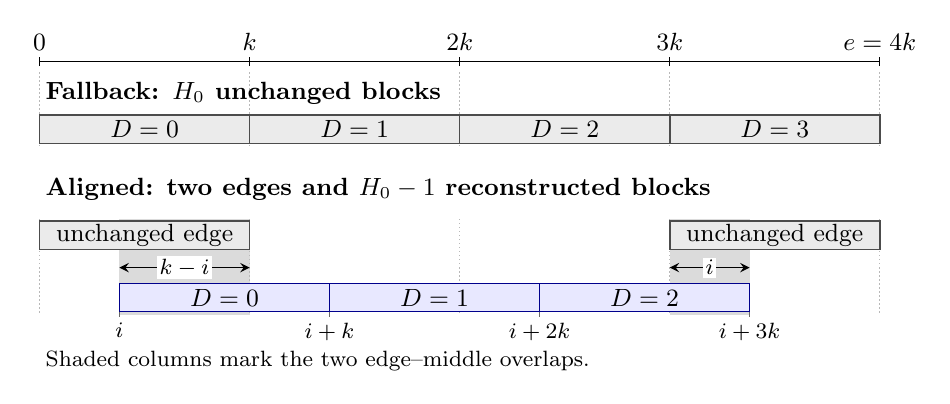
\begin{tikzpicture}[
    x=.22\linewidth,y=8mm,
    font=\small,
    every node/.style={inner sep=2pt},
    original/.style={draw=black!70,fill=black!8,line width=.55pt},
    reconstructed/.style={draw=blue!55!black,fill=blue!9,line width=.55pt},
    overlap/.style={fill=black!14,draw=none},
    guide/.style={draw=black!28,densely dotted,line width=.45pt}
  ]
    \def\blockoffset{.38}

    \draw[line width=.55pt] (0,5.15) -- (4,5.15);
    \foreach \x/\lab in {0/0,1/k,2/2k,3/3k,4/{e=4k}} {
      \draw (\x,5.08) -- (\x,5.22);
      \node[above] at (\x,5.23) {$\lab$};
      \draw[guide] (\x,4.98) -- (\x,3.78);
    }

    \node[anchor=west,font=\small\bfseries] at (0,4.65)
      {Fallback: $H_0$ unchanged blocks};
    \foreach \D in {0,1,2,3} {
      \draw[original] (\D,3.85) rectangle ({\D+1},4.30);
      \node at ({\D+.5},4.075) {$D=\D$};
    }

    \node[anchor=west,font=\small\bfseries] at (0,3.12)
      {Aligned: two edges and $H_0-1$ reconstructed blocks};

    \path[overlap] (\blockoffset,1.13) rectangle (1,2.65);
    \path[overlap] (3,1.13) rectangle ({3+\blockoffset},2.65);
    \foreach \x in {0,1,2,3,4} {
      \draw[guide] (\x,2.65) -- (\x,1.13);
    }
    \draw[original] (0,2.17) rectangle (1,2.62);
    \draw[original] (3,2.17) rectangle (4,2.62);
    \node at (.5,2.395) {unchanged edge};
    \node at (3.5,2.395) {unchanged edge};

    \foreach \D in {0,1,2} {
      \draw[reconstructed]
        ({\blockoffset+\D},1.18)
        rectangle ({\blockoffset+\D+1},1.63);
      \node at ({\blockoffset+\D+.5},1.405) {$D=\D$};
    }
    \foreach \D/\lab in {0/i,1/{i+k},2/{i+2k},3/{i+3k}} {
      \draw[black!60] ({\blockoffset+\D},1.10)
        -- ({\blockoffset+\D},1.18);
      \node[below,font=\footnotesize] at ({\blockoffset+\D},1.10)
        {$\lab$};
    }

    \draw[<->,>=stealth,line width=.5pt]
      (\blockoffset,1.88) -- (1,1.88)
      node[midway,font=\footnotesize,fill=white,inner sep=1pt] {$k-i$};
    \draw[<->,>=stealth,line width=.5pt]
      (3,1.88) -- ({3+\blockoffset},1.88)
      node[midway,font=\footnotesize,fill=white,inner sep=1pt] {$i$};
    \node[anchor=west,font=\footnotesize] at (0,.40)
      {Shaded columns mark the two edge--middle overlaps.};
  \end{tikzpicture}
  \endgroup
  \caption{Aligned and fallback coverage of one macro-interval, translated
    to $[0,e)$. The schematic uses $H_0=4$ and $0<i<k$; every bar denotes
    a half-open interval of length $k$. In general, $e=kH_0$, and the
    middle blocks, with starts $i+Dk$ for $0\le D<H_0-1$, cover
    $[i,e-k+i)$. The unchanged edges $[0,k)$ and $[e-k,e)$ complete the
    coverage. Their overlaps with the middle union are $[i,k)$ and
    $[e-k,e-k+i)$, of lengths $k-i$ and $i$. All blocks lie in $[0,e)$.
    The fallback blocks partition $[0,e)$; at $i=0$, the first middle
    block duplicates the left edge.}
  \label{fig:block-allocation}
\end{figure}
